%TODO: add the analysis part after we remeasure the circuit
%TODO: replot the graph in the first part and recheck the values
\paragraph{Analysis 1}\hfill
\\
\phantom{ } After we connected the circuit in Graph 4.1.1 in the lab instruction, we detected a waveform on our oscilloscope. To calculate its time constant accurately, we need as many data as possible. According to the instruction, we recorded 10 points separately for the original circuit, two-stage and three-stage. When we were selecting our testing points, we tried to pick more where the voltage rose(or fell) more rapidly with time. Also, we noticed that the measurements were not stable on the oscilloscope if its value was too small, so we paused the screen on random to record a relatively accurate number.\\
\phantom{ } When we were measuring the voltages and their according time, we used the Cursor whose type was time and took Channel 2 as its source. We settle one of the cursor at start point of a rising or falling action, and moved the other cursor slightly. We also scaled the width of the waveform to get a more accurate move.\\
\phantom{ } Our recordings for the original circuit are shown in the table below.
\paragraph{Experimental Results}
\begin{table}[htbp]\centering
	\renewcommand\arraystretch{1.5}
	\begin{tabular}{lcl}
		\toprule
		No		&Voltage(V)	&time(ms)	\\
		\midrule
		1		&0.512		&16.0		\\
		
		2		&0.880		&32.0		\\
		
		3		&1.20		&44.0		\\
		
		4		&1.52		&60.0		\\
		
		5		&1.92		&80.0		\\
		
		6		&2.28		&100		\\
		
		7		&2.56		&116		\\
		
		8		&2.60		&124		\\
		
		9		&3.68		&216		\\
		
		10		&4.61		&364		\\
		\bottomrule
	\end{tabular}\\
\end{table}
\phantom{ } Then we apply the data in Excel, we get a plot[\ref{fig:2.1}]:\\
\begin{figure}[htbp]
	\centering %居中
	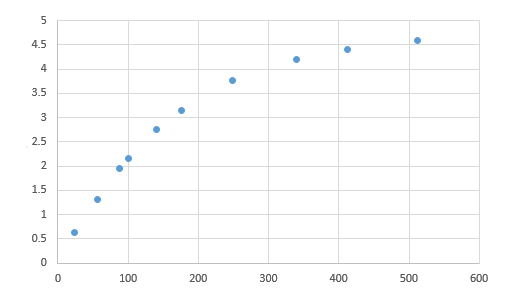
\includegraphics[width=\linewidth]{images/2_1.PNG} %宽度,文件地址
	\caption{plot on the Voltage of capacitor in the original circuit with time.} %标题
	\label{fig:2.1} %标记(引用时用)
\end{figure}\\
\phantom{ } As the instruction suggested, we made the x-axis(time) into logarithmic and plot again[\ref{fig:2.2}] :\\
\begin{figure}[htbp]
	\centering %居中
	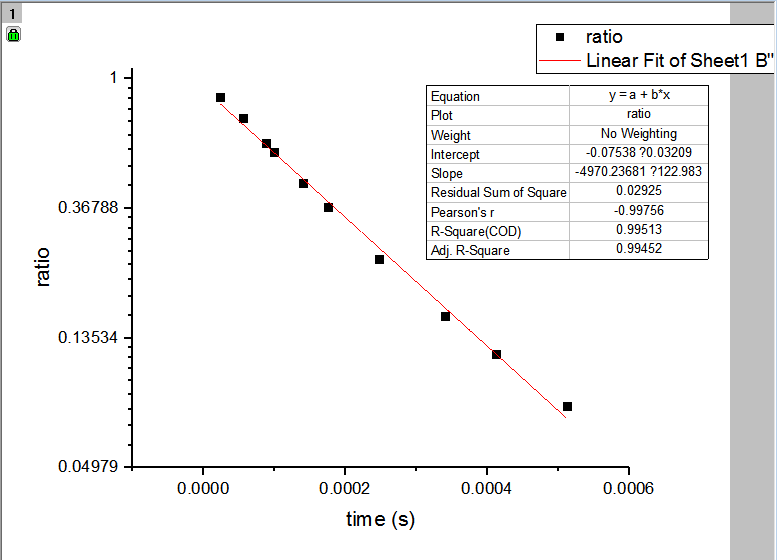
\includegraphics[width=\linewidth]{images/2_2.PNG} %宽度,文件地址
	\caption{plot on the Voltage of capacitor in the original circuit with logarithmic time.} %标题
	\label{fig:2.2} %标记(引用时用)
\end{figure}
\phantom{ } Then we fit a linear line to this plot, and we get a slope of 1.35.
we get its inverse 0.74. Also, we calculated the theoretic value for $\tau$ and got\\
$\tau = RC = 10k\Omega * 0.01\mu F = 0.1ms$, which led to a \% error.
\paragraph{Analysis 2}\hfill
\\
\phantom{ } To finish this analysis, we built a two-stage circuit and then a three-stage circuit. Our two-stage circuit is built according to graph[\ref{fig:2.3}]:\\
\begin{figure}[htbp]
	\centering %居中
	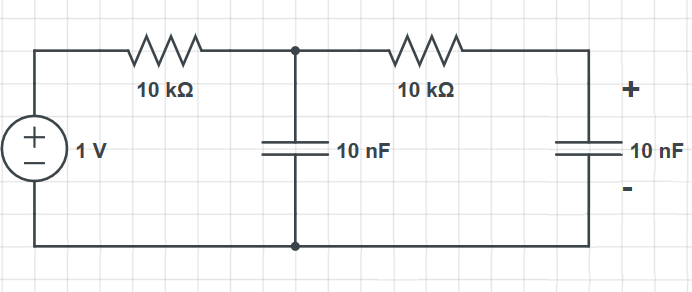
\includegraphics[width=\linewidth]{images/2_3.PNG} %宽度,文件地址
	\caption{the circuit graph of two-stage circuit} %标题
	\label{fig:2.3} %标记(引用时用)
\end{figure}
\phantom{ } In the same way as in the original circuit, we measure 10 points to compute its time constant.
\begin{table}[htbp]\centering
	\renewcommand\arraystretch{1.5}
	\begin{tabular}{lcl}
		\toprule
		No		&Voltage(V)	&time(ms)	\\
		\midrule
		1		&0.400		&60.0		\\
		 
		2		&0.960		&130		\\
		 
		3		&1.56		&210		\\
		 
		4		&1.92		&260		\\
		 
		5		&2.60		&370		\\
		 
		6		&2.88		&430		\\
		 
		7		&3.36		&540		\\
		 
		8		&3.68		&620		\\
		 
		9		&4.32		&880		\\
		 
		10		&4.84		&1330		\\
		\bottomrule
	\end{tabular}
\end{table}
\phantom{ } We then get the time constant of two-stage 
$\tau = $.\\ And according to the circuit graph and some prelab exercise, we can easily compute
the theoretical value of time constant in this case:\\
$\tau = $ and the percent error $error = \%$.\\
\phantom{ } Our three-stage circuit was built based on graph[\ref{fig:2.4}]\\
\begin{figure}[htbp]
	\centering %居中
	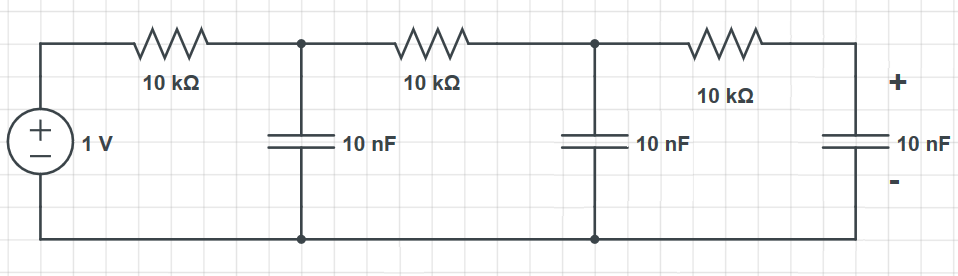
\includegraphics[width=\linewidth]{images/2_4.PNG} %宽度,文件地址
	\caption{the circuit graph of three-stage circuit} %标题
	\label{fig:2.4} %标记(引用时用)
\end{figure}
\phantom{ } And our measure points are listed below:\\
\begin{table}[htbp]\centering
	\renewcommand\arraystretch{1.5}
	\begin{tabular}{lcl}
		\toprule
		No		&Voltage(V)	&time(ms)	\\
		\midrule
		1		&0.560		&0.0		\\
		
		2		&0.720		&140		\\
		
		3		&1.20		&270		\\
		
		4		&1.68		&400		\\
		
		5		&2.32		&580		\\
		
		6		&2.64		&680		\\
		
		7		&3.08		&850		\\
		
		8		&3.56		&1090		\\
		
		9		&4.00		&1380		\\
		
		10		&4.28		&1610		\\
		\bottomrule
	\end{tabular}
\end{table}
\phantom{ } We then get the time constant of three-stage 
$\tau = $.\\ And according to the circuit graph and some prelab exercise, we can easily compute
the theoretical value of time constant in this case:\\
$\tau = $ and the percent error $error = \%$.\\


